\documentclass[12pt]{article}
\usepackage[margin=1in]{geometry}
\usepackage{amsmath}
\usepackage{amssymb}
\usepackage{tikz}
\usepackage{pgfplots}
\usepackage{eso-pic}
\pgfplotsset{compat=1.18}

\AddToShipoutPictureBG{%
  \begin{tikzpicture}[remember picture,overlay]
    \foreach \y in {0,1,...,27} {
      \draw[gray!20, very thin] 
        ([yshift=-\y cm]current page.north west) -- 
        ([yshift=-\y cm]current page.north east);
    }
  \end{tikzpicture}
}

\setlength{\parindent}{0pt}
\setlength{\parskip}{8pt}

\title{Week 8: Review of Weeks 1--7}
\author{
	Student: SA\\
	Tutor: Rachel Eglash}
\date{November 4, 2025}

\begin{document}
	
	\maketitle

	\section*{Session 8.3 Homework}
        
        \textbf{Instructions:} Show all work. Circle your final answers.
        
        \subsection*{Topics Covered:}
        \begin{itemize}
            \item Week 3: Inequalities (Compound \& Word Problems)
            \item Week 4: Linear Equations (Forms \& Intercepts)
            \item Week 5: Systems of Linear Equations (Graphing \& Classification)
            \item Week 6: Linear Functions (Slope \& Applications)
            \item Week 7: Systems of Inequalities \& Applications
        \end{itemize}
	    
        \newpage
	
	    \subsection*{Quick Reference: Key Formulas \& Concepts}
	
	        \subsubsection*{Compound Inequalities}
		    	\textbf{AND:} $a < x < b$ (between two values) \\
                \textbf{OR:} $x < a$ OR $x > b$ (outside two values)
	
	        \subsubsection*{Linear Equation Forms}
			    \textbf{Slope-intercept:} $y = mx + b$ \\
                \textbf{Point-slope:} $y - y_1 = m(x - x_1)$ \\
                \textbf{Standard form:} $Ax + By = C$
	
	        \subsubsection*{Finding Intercepts}
	    		\textbf{x-intercept:} Set $y = 0$ and solve for $x$ \\
                \textbf{y-intercept:} Set $x = 0$ and solve for $y$

            \subsubsection*{Slope Formula}
                $m = \displaystyle\frac{y_2 - y_1}{x_2 - x_1}$ \quad or \quad $m = \displaystyle\frac{\text{rise}}{\text{run}} = \displaystyle\frac{\Delta y}{\Delta x}$

            \subsubsection*{Systems Classification}
                \textbf{One solution:} Different slopes \\
                \textbf{No solutions:} Same slope, different y-intercepts (parallel) \\
                \textbf{Infinitely many:} Same slope, same y-intercept (same line)

            \newpage
	
        \section*{Part A: Compound Inequalities}

            \textbf{Problem 1}\\\\
            Solve: $5x - 3 \leq 7$ OR $2x + 1 > 9$

            \vspace{3cm}

            \textbf{(a)} Graph the solution on a number line.

            \vspace{0.5cm}

            \begin{center}
            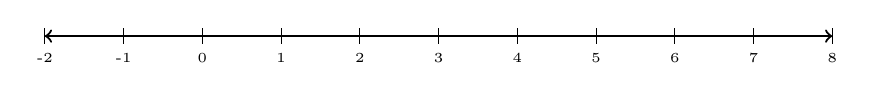
\begin{tikzpicture}
                \draw[<->,thick] (-2,0) -- (8,0);
                \foreach \x in {-2,-1,0,1,2,3,4,5,6,7,8}
                    \draw (\x,0.1) -- (\x,-0.1) node[below] {\tiny\x};
            \end{tikzpicture}
            \end{center}

            \vspace{0.5cm}

            \textbf{(b)} Write the solution in interval notation.

            \newpage

            \textbf{Problem 2}\\\\
            A taxi charges a \$4 base fee plus \$2.50 per mile.\\\\
            You have at most \$30 to spend.\\\\
            Let $m$ = miles traveled (in miles).\\\\
            Assume $m \geq 0$.

            \vspace{0.5cm}

            Write and solve an inequality for $m$.\\\\
            State the greatest whole number of miles you can travel.

            \vspace{3cm}

            \textbf{(a)} Graph the solution on a number line.

            \vspace{0.5cm}

            \begin{center}
            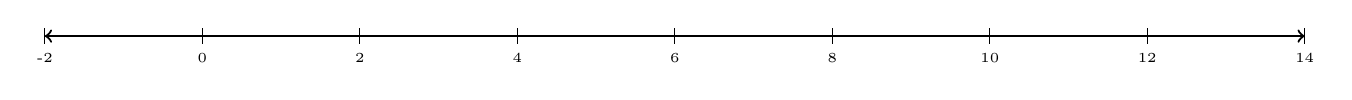
\begin{tikzpicture}
                \draw[<->,thick] (-2,0) -- (14,0);
                \foreach \x in {-2,0,2,4,6,8,10,12,14}
                    \draw (\x,0.1) -- (\x,-0.1) node[below] {\tiny\x};
            \end{tikzpicture}
            \end{center}

            \vspace{0.5cm}

            \textbf{(b)} Write the solution in interval notation.

            \newpage

        \section*{Part B: Linear Equations - Forms \& Intercepts}

            \textbf{Problem 3}\\\\
            Convert to standard form ($Ax + By = C$ where $A$, $B$, $C$ are integers): \\\\
            $y = \displaystyle\frac{3}{4}x - 5$

            \vspace{4cm}

            \textbf{Problem 4}\\\\
            Find the x-intercept and y-intercept of: $5x - 2y = 20$

            \vspace{4cm}

            \textbf{Problem 5}\\\\
            Write the equation of the line through $(2, -3)$ with slope $\displaystyle\frac{1}{2}$ in point-slope form.

            \newpage

        \section*{Part C: Systems - Graphing \& Classification}

            \textbf{Problem 6}\\\\
            Graph each line and classify the system (one solution / no solutions / infinitely many solutions).\\\\
            Find the solution if it exists.

            \begin{align*}
                y &= \frac{1}{2}x + 1\\
                y &= -x + 4
            \end{align*}

            \vspace{1cm}

            \begin{center}
            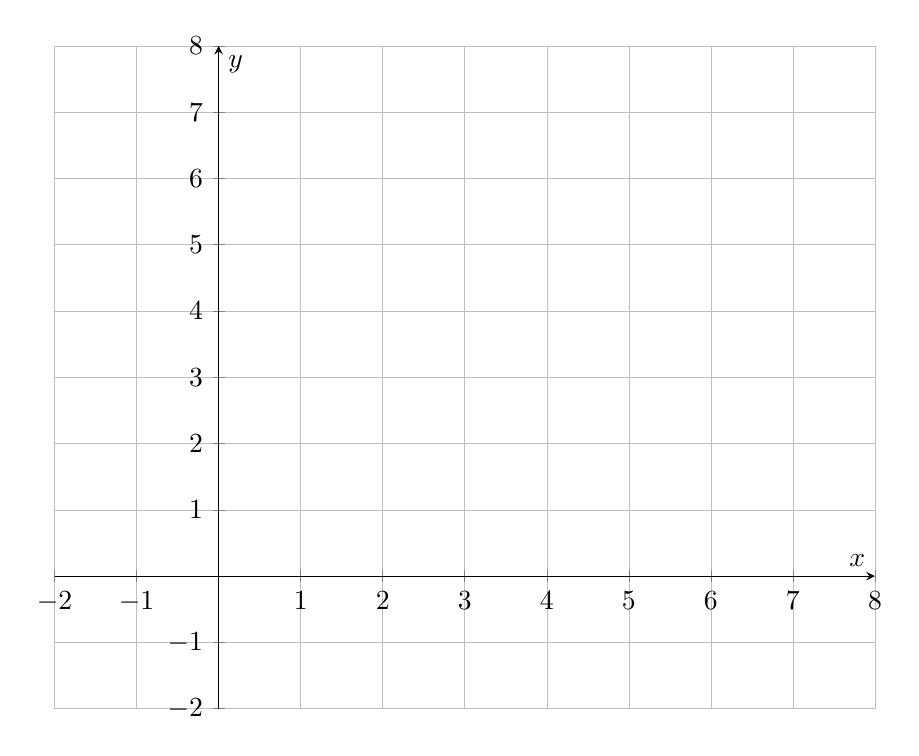
\begin{tikzpicture}
                \begin{axis}[
                    axis background/.style={fill=white},
                    xlabel={$x$},
                    ylabel={$y$},
                    xmin=-2, xmax=8,
                    ymin=-2, ymax=8,
                    xtick={-2,-1,0,1,2,3,4,5,6,7,8},
                    ytick={-2,-1,0,1,2,3,4,5,6,7,8},
                    grid=both,
                    grid style={line width=.1pt, draw=gray!30},
                    major grid style={line width=.2pt,draw=gray!50},
                    width=12cm,
                    height=10cm,
                    axis lines=middle,
                    enlargelimits=false,
                ]
                \end{axis}
            \end{tikzpicture}
            \end{center}

            \newpage

            \textbf{Problem 7}\\\\
            Without graphing, classify the system:

            \begin{align*}
                2x + 3y &= 6\\
                4x + 6y &= 18
            \end{align*}

            \newpage

        \section*{Part D: Slope \& Applications}

            \textbf{Problem 8}\\\\
            A rental car company charges \$45 per day plus \$0.20 per mile.\\\\
            Let $C$ = total cost (in dollars) and $m$ = miles driven.

            \vspace{0.5cm}

            \textbf{(a)} Write an equation for $C$ in terms of $m$ for one day.

            \vspace{4cm}

            \textbf{(b)} Find the cost for driving 150 miles in one day.

            \newpage

        \section*{Part E: Systems of Inequalities}

            \textbf{Problem 9}\\\\
            Graph the system of inequalities and shade the solution region:

            \begin{align*}
                y &\geq x - 2\\
                y &< -\frac{1}{2}x + 4\\
                x &\geq 0\\
                y &\geq 0
            \end{align*}

            \vspace{1cm}

            \begin{center}
            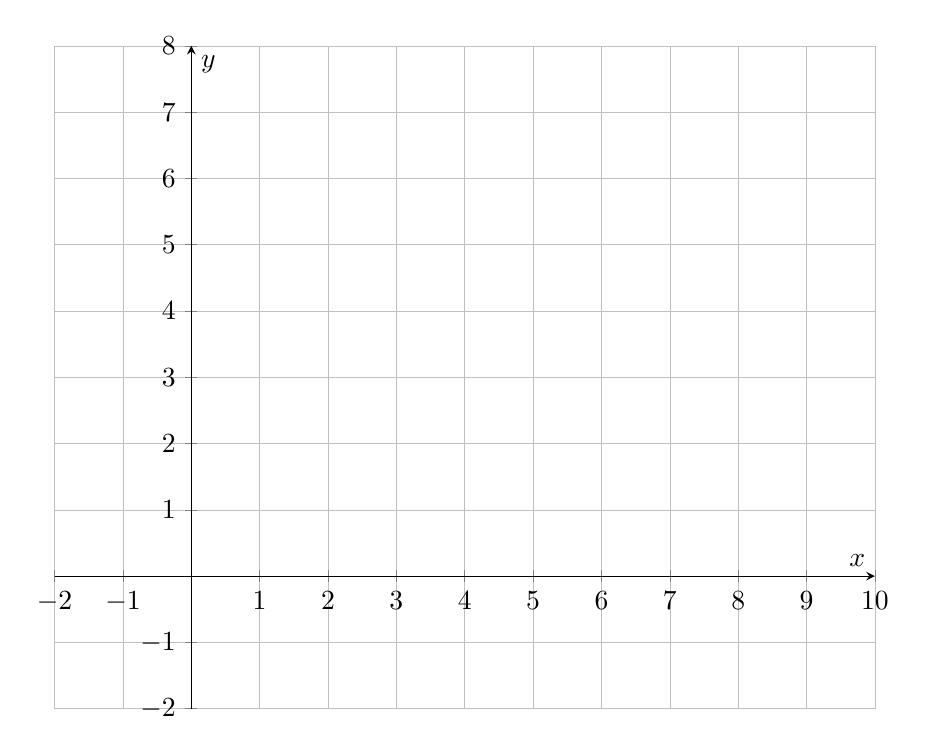
\begin{tikzpicture}
                \begin{axis}[
                    axis background/.style={fill=white},
                    xlabel={$x$},
                    ylabel={$y$},
                    xmin=-2, xmax=10,
                    ymin=-2, ymax=8,
                    xtick={-2,-1,0,1,2,3,4,5,6,7,8,9,10},
                    ytick={-2,-1,0,1,2,3,4,5,6,7,8},
                    grid=both,
                    grid style={line width=.1pt, draw=gray!30},
                    major grid style={line width=.2pt,draw=gray!50},
                    width=12cm,
                    height=10cm,
                    axis lines=middle,
                    enlargelimits=false,
                ]
                \end{axis}
            \end{tikzpicture}
            \end{center}

            \newpage

        \section*{Part F: Applications \& Word Problems}

            \textbf{Problem 10: Mixture Problem}\\\\
            A chemist needs to prepare 80 mL of a 15 $\frac{mg}{mL}$ acid solution.\\\\
            She has a 10 $\frac{mg}{mL}$ acid solution and a 25 $\frac{mg}{mL}$ acid solution.\\\\
            How much of each should she mix?

            \vspace{6cm}

            \textbf{Problem 11: Break-Even Problem}\\\\
            A small business makes custom t-shirts.\\\\
            The fixed costs are \$500 per month.\\\\
            Each t-shirt costs \$8 to produce.\\\\
            Each t-shirt sells for \$20.\\\\
            How many t-shirts must be sold to break even?

            \vspace{6cm}

            \textbf{Problem 12: System Word Problem}\\\\
            Concert tickets are sold in two types: floor seats and balcony seats.\\\\
            There were 200 tickets sold in total.\\\\
            Floor seats cost \$75 each.\\\\
            Balcony seats cost \$50 each.\\\\
            The total revenue was \$12,500.\\\\
            How many of each type of ticket was sold?

\end{document}